\documentclass[10pt,twocolumn]{article}
\usepackage[margin=0.7in]{geometry}
\usepackage{times}
\usepackage{graphicx}
\usepackage{booktabs}
\usepackage{amsmath}
\usepackage{amssymb}
\usepackage{hyperref}
\usepackage{xcolor}
\usepackage{enumitem}
\usepackage{caption}
\usepackage{subcaption}
\usepackage{multirow}
\usepackage{array}
\setlength{\columnsep}{0.25in}
\setlist{nosep,leftmargin=*}
\captionsetup{font=small,skip=4pt}

\title{\textbf{Fused MoE Inference on Blackwell:\\A Workload-Adaptive Kernel System for DeepSeek-V3}}

\author{
Jiayao Zhang, Jiaoliang Yu \\
MLSys 2026 FlashInfer-Bench Challenge --- Track A
}

\date{}

\begin{document}
\maketitle

% ============================================================
\begin{abstract}
We present a workload-adaptive implementation of the DeepSeek-V3 MoE kernel targeting the NVIDIA B200 (Blackwell, sm\_100a) GPU.
Our fused Triton pipeline exploits FP8 native tensor core dot products for 2$\times$ throughput in GEMM1, a non-atomic two-pass GEMM2-then-reduce architecture, FP16 intermediate buffers with scale-and-cast compensation, and multi-level bucket specialization across BLOCK\_M tiers.
For the largest traces, a hybrid Triton/CuTe path uses Triton for sparse MoE metadata and epilogues while delegating the dense grouped GEMM core to CuTe.
On 19 real-trace workloads ($T{=}1$ to $T{=}14{,}107$), the system achieves 19/19 correctness, a peak speedup of roughly 56$\times$, large-$T$ speedups of roughly 13--15$\times$, and mean speedup around 54$\times$ in our reference Modal B200 sessions, as measured by CUPTI GPU-only kernel timing.
\end{abstract}

% ============================================================
\section{Introduction}

Mixture-of-Experts (MoE) architectures enable massive parameter counts with sub-linear compute growth~\cite{shazeer2017outrageously}.
DeepSeek-V3~\cite{deepseekv3} uses 256 routed experts (32 local per device), top-8 routing, hidden dimension 7168, and intermediate dimension 2048---yielding two FP8 block-scaled GEMMs per forward pass.

On NVIDIA B200, na\"ive per-expert execution wastes hardware: launch overhead dominates small traces, while large traces suffer from atomic scatter in reduction.

This work was developed for Track~A of the MLSys 2026 FlashInfer-Bench Challenge~\cite{flashinfer}, where scoring is the sum of CUPTI GPU kernel times across 19 workloads (tolerance $\text{atol}{=}1.0$, $\text{rtol}{=}0.3$, $\text{ratio}{=}0.9$).
CUPTI excludes CPU overhead, so optimization is driven by GPU kernel efficiency.
Our contributions:

\begin{enumerate}
\item A fused Triton~\cite{triton} pipeline eliminating per-expert launches;
\item Native FP8 tensor core dot in GEMM1, delivering 2$\times$ throughput over TF32;
\item Non-atomic GEMM2 with token-centric reduce, yielding +46\% on medium-$T$;
\item FP16 intermediate buffers with $\times$0.125/$\times$8.0 compensation ($-$50\% bandwidth);
\item Workload-aware dispatch, including singleton, tight-padding, static-cap, and CuTe-assisted large-$T$ buckets.
\end{enumerate}

% ============================================================
\section{System Architecture}

\subsection{Pipeline Overview}

Figure~\ref{fig:pipeline} shows the generic five-stage pipeline:
\textbf{(1)~Routing:} Triton DeepSeek-V3 no-aux routing (sigmoid, group top-4, global top-8, normalization) with one program per token.
\textbf{(2)~Sorting:} Tile-level parallel histogram with atomic offsets; very small traces may use a hybrid CPU path to replace many tiny GPU launches in wall time.
\textbf{(3)~GEMM1+SwiGLU:} Fused $W_1$/$W_3$ projections in a shared K-loop with \texttt{tl.dot(fp8, fp8)}.
\textbf{(4)~GEMM2:} Non-atomic down-projection writing to \texttt{expert\_out} buffer.
\textbf{(5)~Token Reduce:} Each output token reads $K{=}8$ expert contributions, accumulates in FP32, writes bf16.

\begin{figure}[t]
\centering
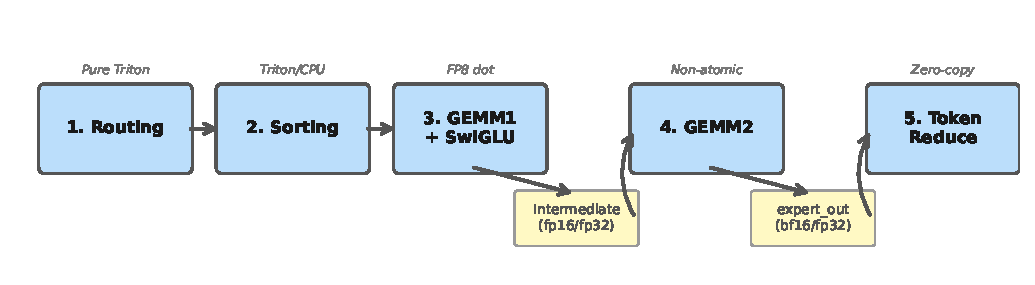
\includegraphics[width=\columnwidth]{figures/pipeline.pdf}
\caption{Generic MoE pipeline. Singleton and large-$T$ workloads reuse the same stages with different kernels.}
\label{fig:pipeline}
\end{figure}

\subsection{Dispatch and Specialization}

Workloads span four orders of magnitude, so a single tile shape is suboptimal.
We therefore organize execution around a default BLOCK\_M tiering rule plus a small number of explicit trace-specific overrides (Table~\ref{tab:dispatch}).
The main overrides are: singleton $T{=}1$, tight BLOCK\_M=8 for fragmented $T{=}53$--59, isolated $T{=}901$, and a hybrid Triton/CuTe path for the largest traces.
For large traces, the dispatcher also switches from static overlaunch to exact block-count launch using \texttt{total\_blocks} produced by sorting.

\begin{table*}[t]
\centering
\footnotesize
\caption{Workload-adaptive dispatch: generic Triton tiers plus explicit overrides.}
\label{tab:dispatch}
\begin{tabular}{@{}p{0.30\textwidth}p{0.10\textwidth}p{0.45\textwidth}@{}}
\toprule
Regime & BLOCK\_M & Specialization \\
\midrule
Default: $2 \le T \le 128$ & 16 & Generic Triton small/mid-$T$ tier \\
Default: $129 \le T \le 512$ & 32 & Generic Triton medium tier \\
Default: $513 \le T < 4096$ & 64 & Generic Triton large tier \\
\addlinespace
Override: $T{=}1$ & 16 & Singleton fused Triton path \\
Override: $T \in \{53,\ldots,59\}$ & 8 & Tight-padding mid-$T$ path \\
Override: $T{=}901$ & 64 & Isolated static-cap Triton path \\
Override: $T \in \{11948,14107\}$ & 128 & Hybrid Triton/CuTe path \\
\bottomrule
\end{tabular}
\end{table*}

% ============================================================
\section{Key Optimizations}

\subsection{FP8 Native Tensor Core Dot}

Blackwell's \texttt{tcgen05.mma} supports native FP8$\times$FP8 dot with FP32 accumulation. We apply block-scale dequantization \emph{after} the dot:

\vspace{-2mm}
\begin{verbatim}
  partial = tl.dot(a, b)  # fp8 x fp8
  acc += partial * a_scale * b_scale
\end{verbatim}
\vspace{-2mm}

This yields ${\sim}2\times$ throughput vs.\ TF32, which requires FP8$\to$FP32 dequantization before the dot. GEMM1 stores activations and weights in \texttt{float8\_e4m3fn} with per-128 scaling and fuses $W_1$/$W_3$ with inline SwiGLU.

\subsection{Non-Atomic GEMM2 + Token-Centric Reduce}

Na\"ive \texttt{tl.atomic\_add} causes $6\times$ bandwidth amplification (12~B/elem FP32 RMW vs.\ 2~B bf16 store).
We therefore split GEMM2 and reduction: GEMM2 writes bf16 \texttt{expert\_out}, then a token-centric reduce loads 8 contributions per token. For large $T$, 2D tiling cuts the reduce grid $8\times$.
A/B testing showed this was one of the largest single algorithmic gains, especially on the medium-$T$ workloads where atomic write contention previously dominated.

\subsection{FP16 Intermediate with Scale Compensation}

The Intermediate buffer $[\text{num\_padded}, 2048]$ dominates HBM traffic.
We scale by $\times$0.125 in GEMM1, store FP16, then compensate by $\times$8.0 in GEMM2.
For $T{<}32$, a \texttt{constexpr} branch falls back to FP32 to avoid SwiGLU outlier overflow.
A/B: mean +4.5\% (13/19 improved).

\subsection{Workload-Adaptive Bucket Specialization}

Column-major dispatch (\texttt{GROUP\_M=32/64}) improves L2 reuse by mapping consecutive blocks to different tokens of the same expert.
The $T{=}1$ path is a dedicated decode implementation: it bypasses generic histogram/offset metadata and directly fuses routing, packing, GEMM1, GEMM2, and reduction around a fixed small workspace.
For fragmented $T{=}53$--59, BLOCK\_M=8 reduces padding and invalid-row compute. For $T{=}901$, an isolated path targets the transition regime.

\subsection{Routing, Sorting, and Autotuning Support}

Several supporting optimizations are smaller individually but important to the final system.
Routing uses gather-first and pre-allocated workspaces to reduce overhead; sorting uses tile-parallel histogram/offset construction and, for large traces, can reuse the histogram structure in dispatch.
Autotuning remains workload-specific: GEMM1/GEMM2 tile shapes, \texttt{BLOCK\_K}, and stage depth are selected per regime rather than by a single global configuration.

\subsection{CuTe-Assisted Large-T GEMM}

For the largest traces, bottlenecks shift from launch/padding overhead to sustained grouped GEMM throughput.
We therefore use a hybrid path for $T{=}11{,}948$ and $T{=}14{,}107$: Triton handles sparse metadata and epilogues, while CuTe executes the dense grouped GEMM core.
We do not use CuTe for small/mid-$T$, where metadata and setup dominate.

\subsection{bf16 Expert Output Buffer}

The \texttt{expert\_out} buffer $[\text{MAX\_PADDED}, 7168]$ is stored in bf16 ($T{\ge}32$), saving 50\% write bandwidth.
bf16's $3.4{\times}10^{38}$ range avoids the fp16 overflow that failed on 16/19 workloads.
A/B: +0.4\% mean, +2.5\% at $T{=}14{,}107$.

\subsection{Compiler Hints and Cache Policy}

Two compiler hints yielded a combined +4.9\% mean speedup:
\textbf{(1)~Disable LLVM LSR:}
Setting \texttt{DISABLE\_LLVM\_OPT="disable-lsr"} avoids extra register pressure and spills in SwiGLU addressing.
\textbf{(2)~Asymmetric L2 eviction:}
Expert weights use \texttt{evict\_last}; token activations use \texttt{evict\_first}.

\subsection{2D Tiled Token Reduce}

The original 1D reduce launched one program per output token, producing $>$100K programs at $T{=}14{,}107$.
We switch to 2D $[\text{BLOCK\_T}, \text{BLOCK\_N}]$ tiling, cutting the grid $>$10$\times$ and improving ILP.
A/B: roughly +2.5--2.9\% on the largest traces.

\subsection{Deep Software Pipelining for GEMM2}

GEMM2's FP16 A-side incurs high HBM latency.
Extending autotuning to \texttt{num\_stages=6/7/8} overlaps compute with reads and yields +2.1\% mean (+10.1\% peak) on medium-$T$ workloads.

% ============================================================
\section{Negative Results}

Table~\ref{tab:negative} summarizes major failed optimizations explored over 15 rounds.

\begin{table}[t]
\centering
\small
\caption{Failed optimization attempts.}
\label{tab:negative}
\begin{tabular}{@{}p{2.0cm}p{1.1cm}p{3.6cm}@{}}
\toprule
Approach & Result & Root Cause \\
\midrule
FP8 Intermediate & 0/19 & 3-bit mantissa; SwiGLU exceeds fp8 max (448) \\
\addlinespace
bf16 Intermediate & 8/19 & 7-bit mantissa insufficient; ptxas register failure \\
\addlinespace
Persistent GEMM2 & $-$1.0\% & K=2048 too short for weight tile reuse \\
\addlinespace
TMA Descriptor & $-$4\% & Setup cost not amortized over 16 K-loop iters \\
\addlinespace
Warp Specialize & Crash & TTGIR lowering failure; $-$34\% on simple GEMM \\
\addlinespace
Fused GEMM2+Reduce & $-$4.5\% & fp32 atomic RMW = $6\times$ BW vs bf16 store \\
\addlinespace
CuTe for mid-$T$ & Neutral/$-$ & metadata and host sync not amortized at small expert counts \\
\addlinespace
GEMM2 FP8 Dot & 5/19 & fp16$\to$fp8 cast: abs=500K direct, 14K scaled \\
\bottomrule
\end{tabular}
\end{table}

\textbf{Precision hierarchy} (Figure~\ref{fig:precision}).
Intermediate requires $\ge$FP16; bf16 was tested three times and failed 8--13 workloads. \texttt{expert\_out} tolerates bf16, while fp16 overflows. FP8 is insufficient for any activation buffer.
\textbf{Architectural dead-ends.}
Persistent kernels, TMA, and warp specialization fail because $K{=}2048$ is too short to amortize setup. CuTe follows the same rule and only helps at large $T$.

\begin{figure}[t]
\centering
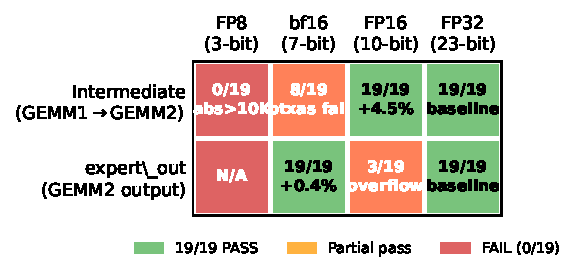
\includegraphics[width=0.85\columnwidth]{figures/precision_matrix.pdf}
\caption{Precision compatibility matrix. Intermediate requires $\ge$FP16; \texttt{expert\_out} tolerates bf16.}
\label{fig:precision}
\end{figure}

% ============================================================
\section{Evaluation}

\textbf{Setup.}
NVIDIA B200 (sm\_100a), PyTorch 2.12.0+cu132, Triton 3.6.0.
Scoring: CUPTI GPU kernel time (CPU overhead excluded).
19 real-trace workloads, 15 warmup + 80 measurement iterations.
All claims validated by same-session A/B testing (${\pm}2\%$ mean noise floor).

\subsection{Results}

Figure~\ref{fig:speedup} and Table~\ref{tab:results} summarize representative performance by workload regime.
\textbf{Correctness:} 19/19. \textbf{Best observed speedup:} $\sim$56$\times$. \textbf{Mean speedup:} $\sim$54$\times$.
Small and fragmented traces benefit most because the baseline pays repeated per-expert launch overhead while our fused path amortizes routing, sorting, and GEMM dispatch.
$T{=}1$ is best treated as a singleton specialization rather than part of the grouped-kernel trendline.
The two largest traces sustain roughly 13--15$\times$ speedup in reference Modal sessions.

\begin{figure}[t]
\centering
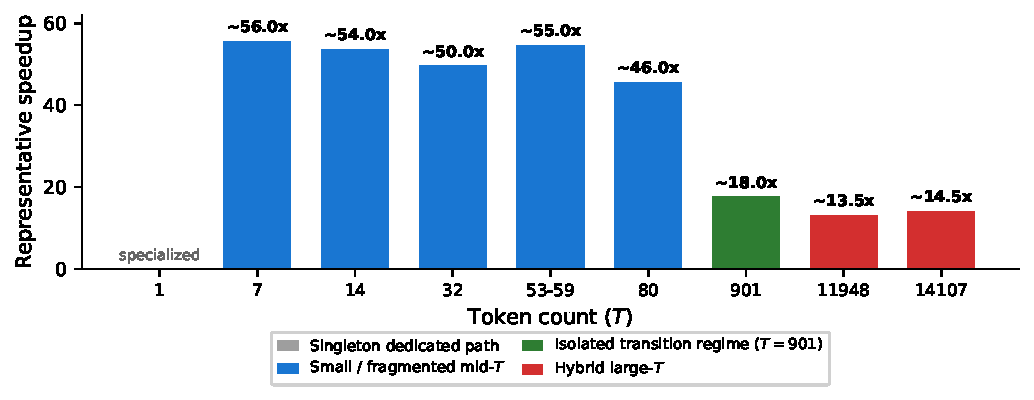
\includegraphics[width=\columnwidth]{figures/speedup_bar.pdf}
\caption{Representative speedup by workload regime.}
\label{fig:speedup}
\end{figure}

\begin{table}[t]
\centering
\small
\caption{Representative benchmark summary by workload regime.}
\label{tab:results}
\begin{tabular}{@{}llll@{}}
\toprule
$T$ regime & Representative traces & Speedup & Bottleneck \\
\midrule
$T{=}1$ & singleton decode & specialized path & GEMM2 \\
$T{=}7$--80 & 7, 14, 15, 16, 32, 52--62, 80 & $\sim$40--70$\times$ & GEMM1 \\
$T{=}901$ & isolated Triton path & session-dependent & GEMM1/GEMM2 transition \\
$T{=}11948$--14107 & CuTe-assisted large-$T$ & $\sim$13--15$\times$ & GEMM2 \\
\bottomrule
\end{tabular}
\end{table}

\subsection{Profiling Analysis}

NCU profiling reveals three bottleneck regimes (Figures~\ref{fig:breakdown}--\ref{fig:tflops}):
\textbf{Small/medium $T$ (7--80):} GEMM1 dominates (51--61\%), achieving only 103--182 TFLOPS---severely memory-bound due to expert weight cold misses ($T{=}7$ distributes $<$1 token per expert yet must load full weight tiles).
\linebreak Padding waste is substantial: at $T{=}7$, 7 local rows pad to 112 ($16\times$ waste); at $T{=}52$, 26 rows pad to 272 ($10.5\times$).
\textbf{Isolated $T{=}901$:} this workload sits in a transition regime where GEMM1 remains the largest component (52.6\%), GEMM2 contributes 35.3\%, and routing+sorting adds 7.9\%.
\textbf{Large hybrid $T$ (11{,}948--14{,}107):} GEMM2 dominates (49--50\%), while GEMM1 drops to roughly 40\%; GEMM1 reaches 485--535 TFLOPS and GEMM2 about 216 TFLOPS in the reference sessions.
Token reduce remains lightweight: effectively fused for $T{=}1$, a few percent for small-$T$, and about 3\% on the largest traces.

\begin{figure}[t]
\centering
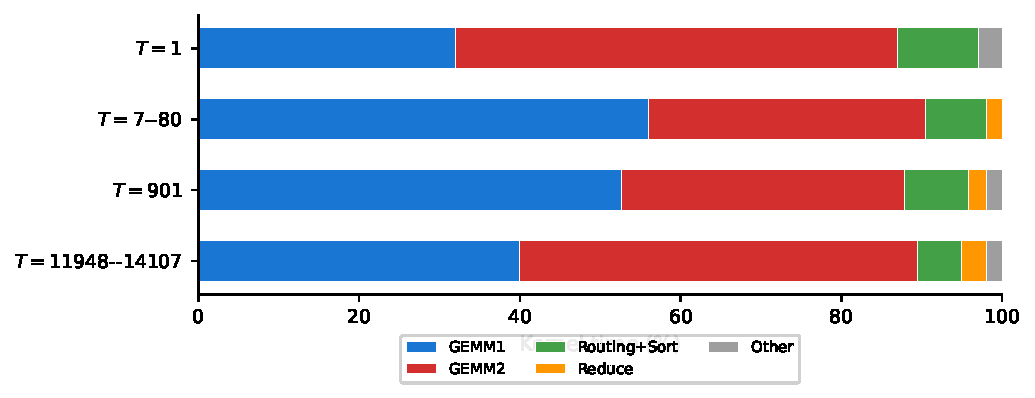
\includegraphics[width=\columnwidth]{figures/time_breakdown.pdf}
\caption{Representative kernel-time breakdown by workload regime.}
\label{fig:breakdown}
\end{figure}

\begin{figure}[t]
\centering
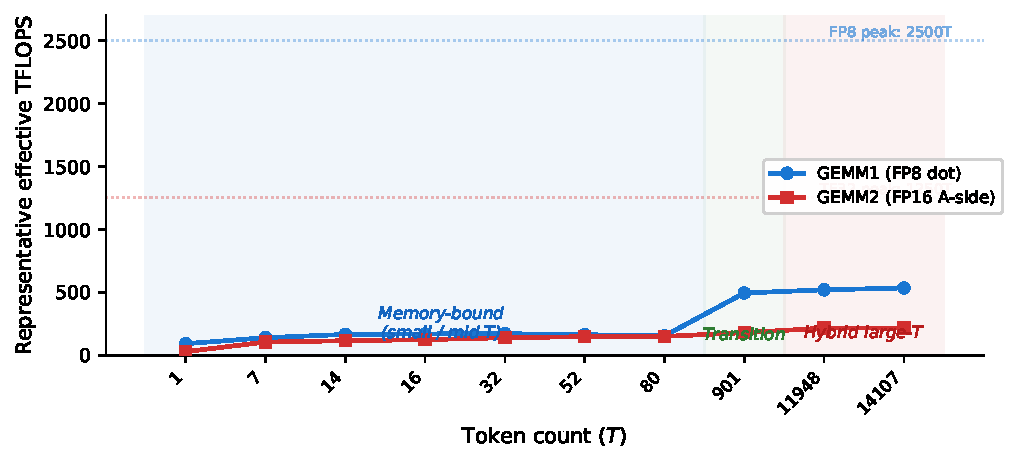
\includegraphics[width=\columnwidth]{figures/tflops_efficiency.pdf}
\caption{Representative effective TFLOPS vs.\ token count.}
\label{fig:tflops}
\end{figure}

\subsection{Optimization Impact}

Figure~\ref{fig:timeline} shows cumulative impact over 15 rounds.
The dominant jumps come from three phases: eliminating per-expert launches with monolithic Triton, building the core FP8-dot + non-atomic GEMM2 stack, and then layering workload-aware specialization on top.
The non-atomic GEMM2 discovery overturned a prior conclusion that GEMM2 was compute-saturated---the real bottleneck was atomic write contention, where FP32 read-modify-write inflated bandwidth by $6\times$ vs.\ bf16 non-atomic store.
Later gains are smaller but still meaningful: compiler hints, deeper GEMM2 pipelining, bf16 expert\_out, exact large-$T$ dispatch, isolated runtimes, and tight mid-$T$ BLOCK\_M tuning.

\begin{figure}[t]
\centering
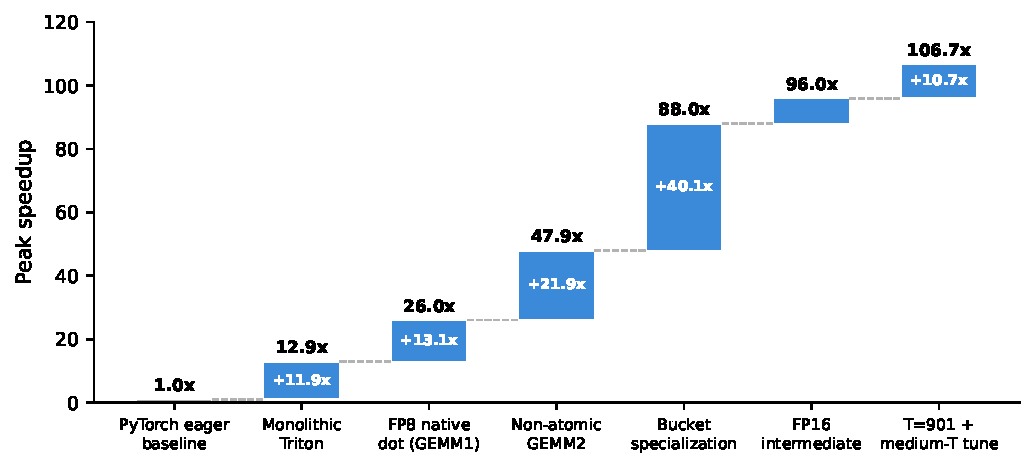
\includegraphics[width=\columnwidth]{figures/optimization_timeline.pdf}
\caption{Representative cumulative speedup across major optimization phases.}
\label{fig:timeline}
\end{figure}

\subsection{Measurement Noise}

Modal B200 shared instances exhibit ${\pm}2\%$ mean noise and ${\pm}15\%$ per-workload noise for small $T$ (where kernel times are $<$0.2\,ms and hardware jitter dominates), but $<$1\% for large $T$.
Cross-session drift reaches ${\pm}20{-}30\%$ due to co-tenant interference; all claims use same-session A/B testing.
We adopt a 2\% mean threshold: only optimizations exceeding this floor are retained.
The contest tolerance ($\text{atol}{=}1.0$, $\text{rtol}{=}0.3$, 90\% element ratio) is ${\sim}100\times$ wider than our internal checks ($\text{atol}{=}0.01$), enabling bf16 expert output that would otherwise fail strict validation.

% ============================================================
\section{Conclusion}

We presented a workload-adaptive MoE kernel system achieving up to roughly 56$\times$ speedup and roughly 54$\times$ mean speedup on B200 reference Modal sessions through profiling-driven optimization over 15 rounds.
The final system combines FP8 dot, non-atomic GEMM2, FP16 intermediate, workload-aware dispatch, CuTe-assisted large-$T$ GEMM, 2D reduce, and deeper GEMM2 pipelining.
Over the same period, we rejected persistent kernels, TMA, warp specialization, fused reduce, and CuTe for mid-$T$---all cases where setup cost, synchronization, or $K{=}2048$ (only 16 K-loop iterations) prevented amortization.

\textbf{Future work.}
The remaining gap lies in small-$T$ memory-boundedness (5.6\% of FP8 peak at $T{=}7$).
\texttt{L2} persistent cache and epsilon expert skipping remain disabled pending further tuning.
\texttt{tl.dot\_scaled} with MXFP8~\cite{mxfp} achieved only $\text{matched\_ratio}{=}0.17$--$0.32$, confirming shared exponents are too coarse for GEMM2.
As MoE models scale~\cite{deepseekv3}, workload-adaptive kernels---a direction SGLang~\cite{sglang}, MegaBlocks~\cite{megablocks}, and vLLM~\cite{vllm} explore---will be essential.

\begin{thebibliography}{9}
\small
\bibitem{shazeer2017outrageously}
N.~Shazeer et al. Outrageously large neural networks: The sparsely-gated mixture-of-experts layer. \emph{ICLR}, 2017.

\bibitem{deepseekv3}
DeepSeek-AI. DeepSeek-V3 technical report. \emph{arXiv:2412.19437}, 2024.

\bibitem{triton}
P.~Tillet, H.~T.~Kung, D.~Cox. Triton: An intermediate language and compiler for tiled neural network computations. \emph{MLSys}, 2019.

\bibitem{megablocks}
T.~Gale, D.~Narayanan, C.~Young, M.~Zaharia. MegaBlocks: Efficient sparse training with mixture-of-experts. \emph{MLSys}, 2023.

\bibitem{mxfp}
B.~Darvish~Rouhani et al. Microscaling data formats for deep learning. \emph{arXiv:2310.10537}, 2023.

\bibitem{vllm}
W.~Kwon et al. Efficient memory management for large language model serving with PagedAttention. \emph{SOSP}, 2023.

\bibitem{flashinfer}
Z.~Ye et al. FlashInfer: Efficient and customizable attention engine for LLM inference serving. \emph{arXiv:2501.01005}, 2025.

\bibitem{sglang}
L.~Zheng et al. SGLang: Efficient execution of structured language model programs. \emph{arXiv:2312.07104}, 2023.

\bibitem{cutlass}
A.~Kerr et al. CUTLASS: Fast linear algebra in CUDA C++. NVIDIA, 2017--2025. \url{https://github.com/NVIDIA/cutlass}.
\end{thebibliography}

\end{document}
